\section{Dataset and Data Engineering}
\label{sec:dataset}

The experiments use \dataset{} for repeatable evaluation of edge-cloud IoT offloading under stress. It is a realistic synthetic benchmark generated for this project with temporal workload phases, correlated channel states, edge pressure, cloud load, and fault windows. The paper treats it as the final benchmark dataset for the reported experiments.

The dataset contains 100,000 task rows, 50 edge nodes, 10 cloud nodes, and 1,000 timesteps. The six CSV files describe task records, static edge nodes, per-timestep edge state, per-timestep network state, static cloud nodes, and per-timestep cloud state. Table~\ref{tab:dataset_schema} summarizes the files.

\begin{table*}[!t]
\centering
\caption{\dataset{} files and schema roles.}
\label{tab:dataset_schema}
\scriptsize
\resizebox{\textwidth}{!}{%
\begin{tabular}{@{}lrrl@{}}
\toprule
File & Rows & Columns & Role \\
\midrule
\texttt{dataset\_A.csv} & 100,000 & 23 & Task records, device/task properties, arrival time, assigned edge, dependency and risk flags. \\
\texttt{edge\_nodes.csv} & 50 & 8 & Static edge-node capacity, tier, renewable-power flag, and location zone. \\
\texttt{edge\_state.csv} & 50,000 & 10 & Per-timestep edge CPU, memory, queue, latency, energy, failure, degradation, and isolation state. \\
\texttt{network\_state.csv} & 1,000 & 11 & Per-timestep uplink/downlink bandwidth, delay, packet loss, load, SNR, outage, congestion, and jitter. \\
\texttt{cloud\_nodes.csv} & 10 & 6 & Static cloud region, CPU, memory, bandwidth, and SLA tier. \\
\texttt{cloud\_state.csv} & 10,000 & 9 & Per-timestep cloud CPU, memory, queue, latency, maintenance, overload, and cold-start state. \\
\bottomrule
\end{tabular}}
\end{table*}

\begin{table*}[!t]
\centering
\caption{Reproducibility package components for the reported benchmark.}
\label{tab:reproducibility_manifest}
\scriptsize
\begin{tabularx}{\textwidth}{@{}lXX@{}}
\toprule
Component & Role & Release/check status \\
\midrule
Dataset generator & Creates the task, edge, network, and cloud CSV files with temporal bursts, correlated channel state, and fault windows. & Project artifact; generator-native parameters documented with the dataset. \\
Six CSV files & Provide tasks, edge nodes, edge state, network state, cloud nodes, and cloud state for repeatable evaluation. & Row counts and column schemas are checked before training. \\
Temporal split protocol & Defines train, validation, gap, and held-out test windows by arrival timestep. & Fixed in the manuscript and reused across all policies. \\
Label-generation logic & Computes edge/cloud latency estimates, SLA flags, and selected-path rejection outcomes. & Kept outside the Stage-1 feature matrix to avoid target leakage. \\
Analysis workflow and figure exporter & Produce model outputs, tables, and manuscript figures from the same held-out actions. & Reused for final tables and diagnostics. \\
Checksum manifest & Verifies file identity for the benchmark package and records CSV schema size. & Exported with the manuscript bundle as \texttt{dataset\_checksums.csv}. \\
\bottomrule
\end{tabularx}
\end{table*}


\subsection{Temporal Workload Phases}

The task generator creates workload phases instead of sampling every row independently. Normal periods are mixed with morning and evening bursts, emergency bursts, firmware rollout windows, industrial telemetry surges, and video or AI-heavy peaks. Multiple tasks can arrive at the same timestep and create pressure on queues, bandwidth, and available compute. The resulting offloading problem is harder than choosing between edge and cloud from isolated task descriptors.

Task size uses a mixture of lognormal and heavy-tailed samples. CPU cycles, memory demand, deadline, priority, security requirements, and battery state are correlated with task type and device type. For example, emergency tasks have tight deadlines, firmware updates have larger transfer sizes but relaxed deadlines, and AI/video tasks tend to have heavier compute and memory requirements. These correlations matter because a model trained on uncorrelated synthetic features can learn shortcuts that do not survive even modest workload realism.

\subsection{Network, Edge, and Cloud State}

Network state is generated as a time-correlated process. Congestion, outage, and jitter windows affect packet loss, delay, available bandwidth, and SNR for multiple consecutive timesteps, which is closer to operational behavior than independent packet-loss draws at every row. Edge state also carries temporal pressure: local task arrivals increase queue length, reduce effective CPU and memory availability, and drain energy. Failures and degradation can occur in clusters, and some nodes partially recover after a fault window.

Cloud state is also stateful. Maintenance, overload, and cold starts can raise queue and latency for multiple timesteps. The generator does not make cloud unattractive by construction. The benchmark includes edge-favorable, cloud-favorable, and ambiguous cases, since a dataset where one destination is almost always best would not test policy learning.

The channel model used by the feature pipeline can be interpreted through an effective bandwidth term:
\begin{equation}
B^{\mathrm{eff}}_t =
\max\left(\epsilon_B,
B^{\mathrm{up}}_t(1-\ell_t)(1-o_t)(1-\xi_t)\right),
\label{eq:effective_bandwidth}
\end{equation}
where $B^{\mathrm{up}}_t$ is uplink bandwidth, $\ell_t\in[0,1]$ is packet-loss rate, $o_t\in\{0,1\}$ is an outage indicator, and $\xi_t\in[0,1]$ is a clipped jitter/congestion discount. The floor $\epsilon_B>0$ prevents non-positive bandwidth in downstream pressure ratios. The term is not a physical radio simulator. Its role is to expose the learner to interacting bandwidth, loss, outage, and jitter effects instead of treating those quantities as unrelated features.

Queue pressure is also carried over in time. A simplified recurrence is
\begin{equation}
q^e_{j,t+1} =
\max\left(0, q^e_{j,t} + A_{j,t} - \mu^e_{j,t} + \omega_{j,t}\right),
\label{eq:queue_carryover}
\end{equation}
where $A_{j,t}$ is the local arrival count, $\mu^e_{j,t}$ is effective service capacity, and $\omega_{j,t}$ is a signed stress adjustment: degradation or isolation can increase it, while recovery can decrease it. The outer projection preserves the queue invariant $q^e_{j,t}\geq0$. The CSV state tables store the realized values generated by this logic, while the policy observes their effect through edge queue, CPU, memory, energy, network, and cloud-load features.

\begin{figure*}[!t]
\centering
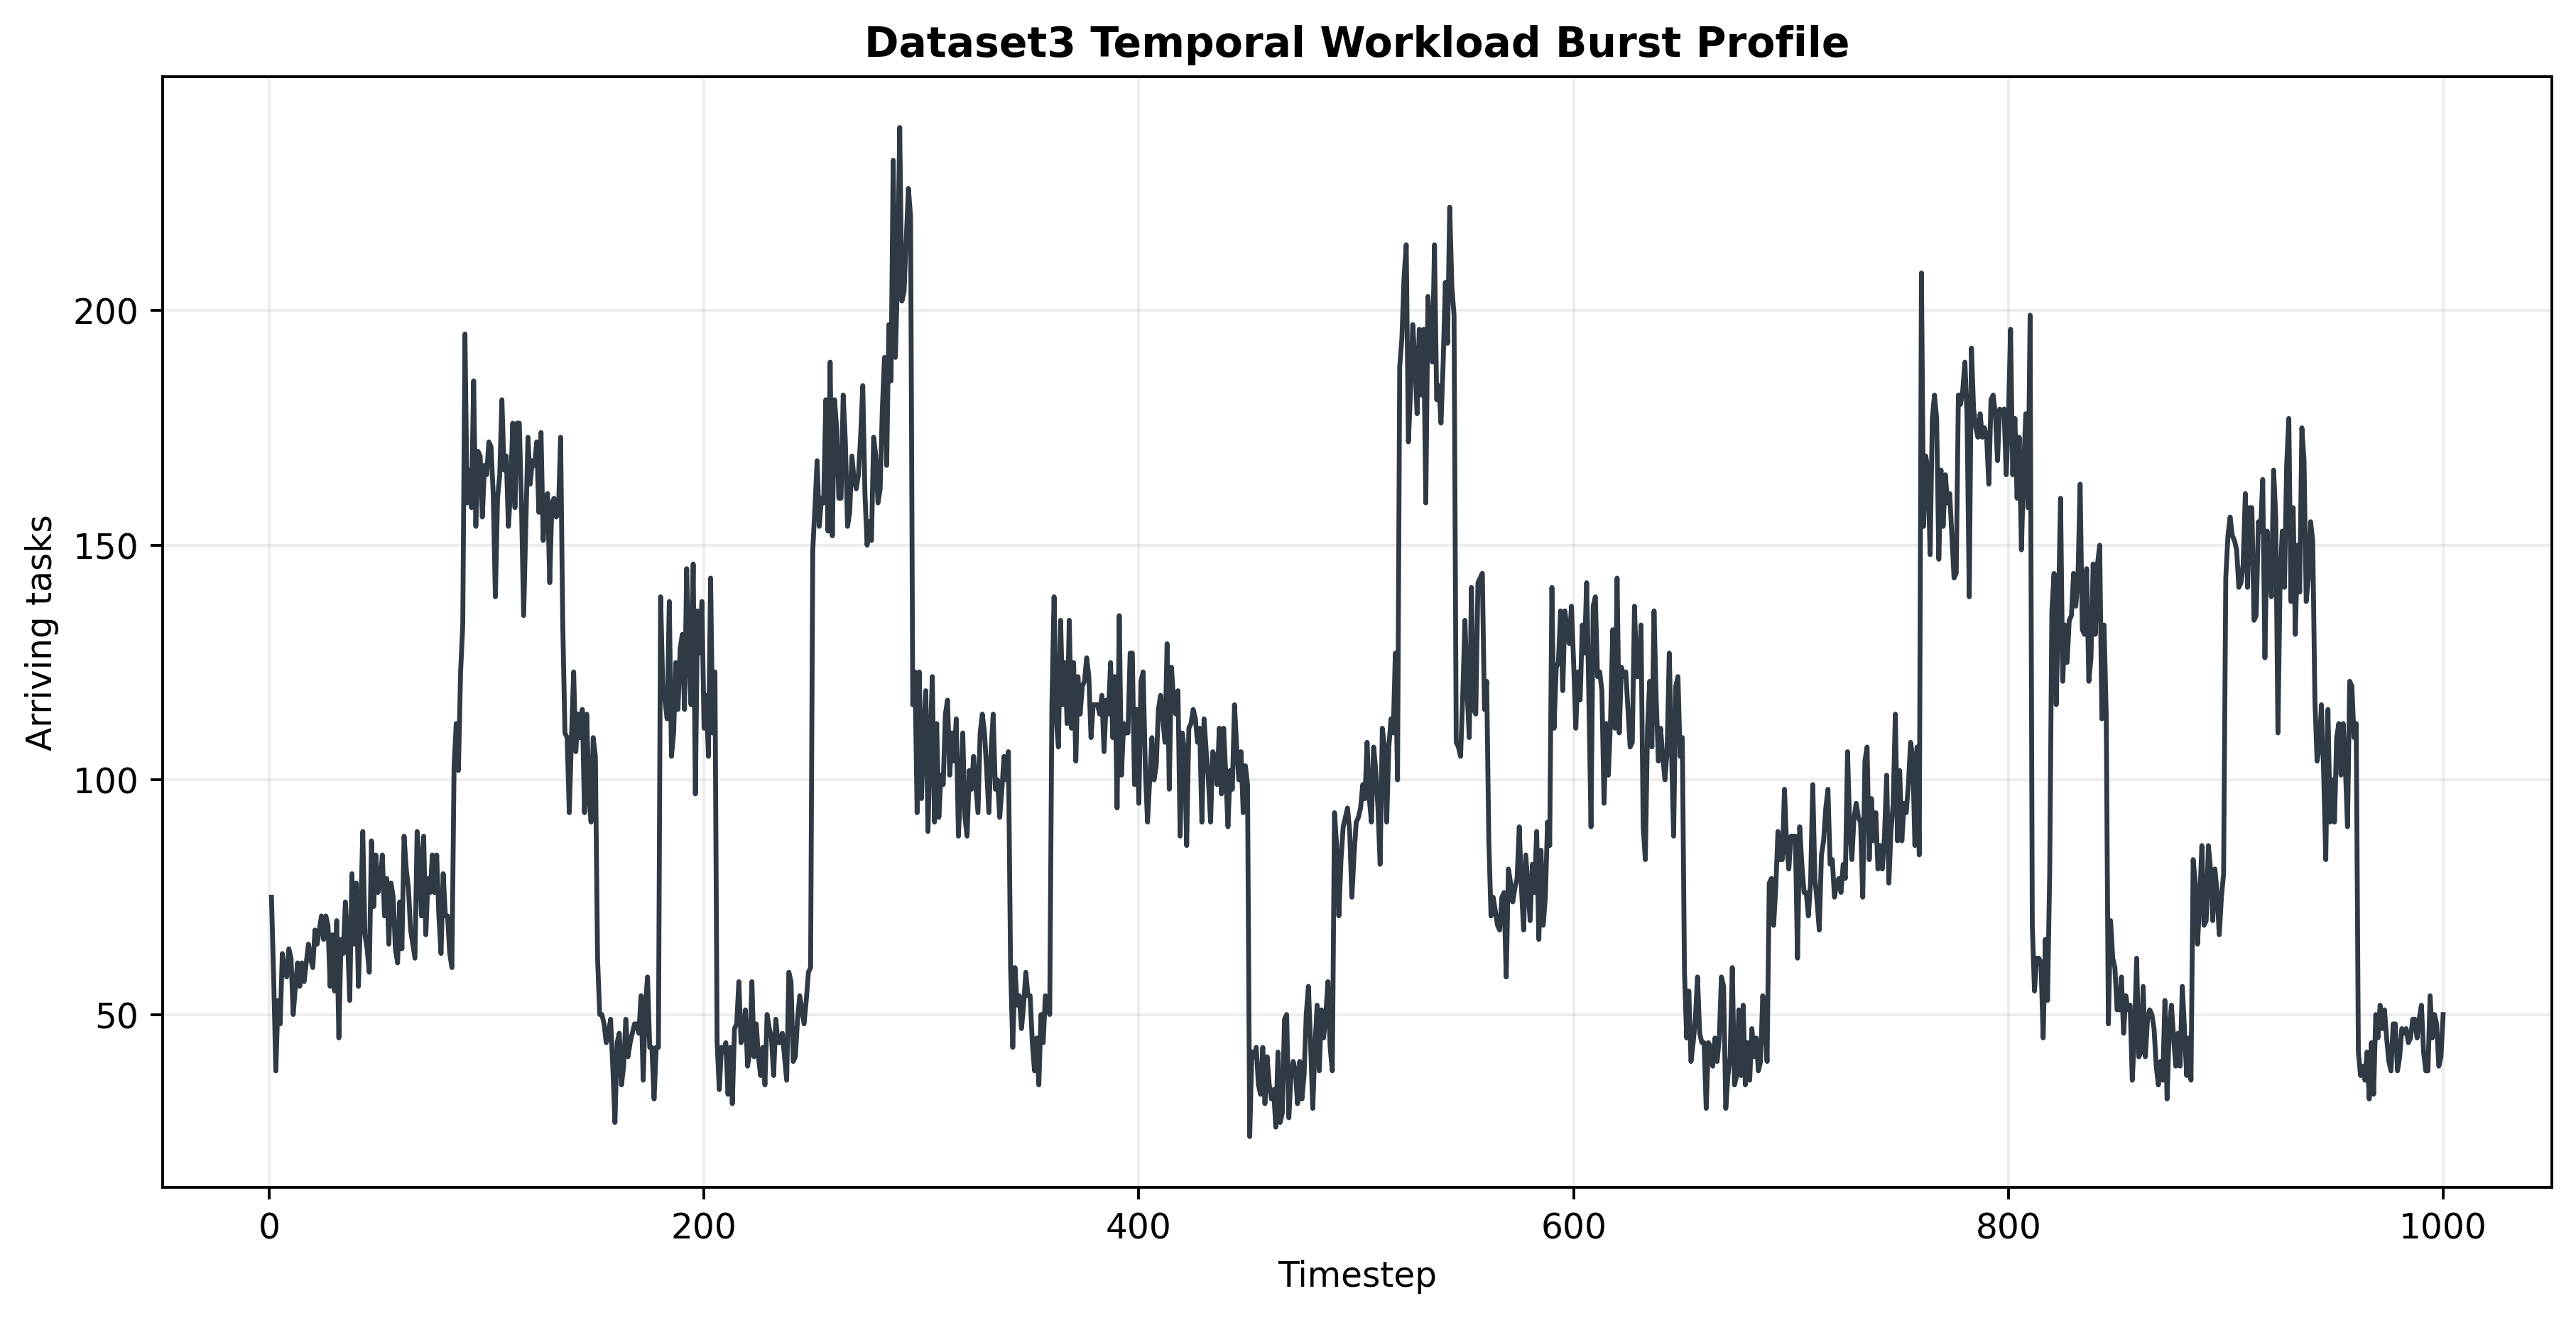
\includegraphics[width=0.90\textwidth]{figures/diagnostics/166_fig_a19_dataset_workload_network_timeline.png}
\caption{Workload and network timeline in \dataset{}, showing burst and stress windows generated for repeatable edge-cloud evaluation.}
\label{fig:dataset_timeline}
\end{figure*}

\subsection{Race-Like Contention Approximation}

The offline benchmark reads precomputed CSV state files, so it does not simulate concurrent state mutation while a policy acts. Instead, \dataset{} approximates race-like pressure through precomputed contention. For each timestep, the generator counts total arrivals, edge-local arrivals, likely cloud-heavy tasks, and recent workload carryover. These values influence edge queues, edge availability, network quality, and cloud queue state. The learned model sees simultaneous arrivals as different from isolated arrivals, even though the benchmark remains a fixed offline dataset.

\subsection{Labels, Features, and Leakage Control}

Labels are produced by computing edge and cloud latency with the same lookup tables used by the final implementation. Rejection and SLA flags are derived outcomes. Sentinel latencies are kept out of the feature matrix to avoid polluting training with artificial extreme values. The Stage-1 feature matrix has 30 columns and is checked against \texttt{features\_raw.shape == (100000, 30)}. The realized rejection label is not included as a Stage-1 input feature.

\begin{table*}[!t]
\centering
\caption{Exact Stage-1 feature list used for offloading model input.}
\label{tab:features}
\scriptsize
\begin{tabularx}{\textwidth}{@{}lX@{}}
\toprule
Group & Included Stage-1 feature names \\
\midrule
Task descriptors & \texttt{task\_size\_mb}, \texttt{cpu\_cycles}, \texttt{memory\_req\_mb}, \texttt{deadline\_ms}, \texttt{priority\_level}, \texttt{energy\_required}, \texttt{security\_sensitivity}, \texttt{task\_type}, \texttt{device\_type}. \\
Task and device flags & \texttt{is\_real\_time}, \texttt{is\_encrypted}, \texttt{is\_low\_battery}, \texttt{has\_dependency}, \texttt{retransmission\_count}. \\
Edge state & \texttt{e\_cpu}, \texttt{e\_mem}, \texttt{e\_queue}, \texttt{e\_energy}, \texttt{e\_fail}, \texttt{e\_deg}. \\
Network/channel state & \texttt{n\_delay}, \texttt{n\_bw}, \texttt{n\_loss}, \texttt{n\_snr}, \texttt{eff\_bw}, \texttt{n\_out}, \texttt{n\_jit}, \texttt{n\_cong}. \\
Cloud state & \texttt{c\_cpu}, \texttt{c\_over}. \\
Feature-label boundary & The Stage-1 feature matrix has 30 columns and is checked against \texttt{features\_raw.shape == (100000, 30)}. Label-only fields such as \texttt{rejection\_flag}, \texttt{rejected}, \texttt{sla\_violated}, \texttt{edge\_latency}, and \texttt{cloud\_latency} are not Stage-1 input features. \\
\bottomrule
\end{tabularx}
\end{table*}


The label-generation logic can use additional task and state fields to compute edge latency, cloud latency, SLA violation, and rejection outcomes. Those derived outcomes are then kept outside the Stage-1 feature vector. The model can observe operational predictors such as queue, SNR, outage, and cloud overload without directly receiving the target labels used for evaluation.

The temporal split is purged to reduce leakage across adjacent timesteps. Training uses arrivals up to timestep 700. Timesteps 701--715 are ignored as a gap. Validation uses timesteps 716--850. Timesteps 851--865 are ignored as the second gap. The final test split uses timesteps 866--1000. The scaler is fit only on the training rows, and validation/test rows are transformed using that scaler.

\begin{figure}[!t]
\centering
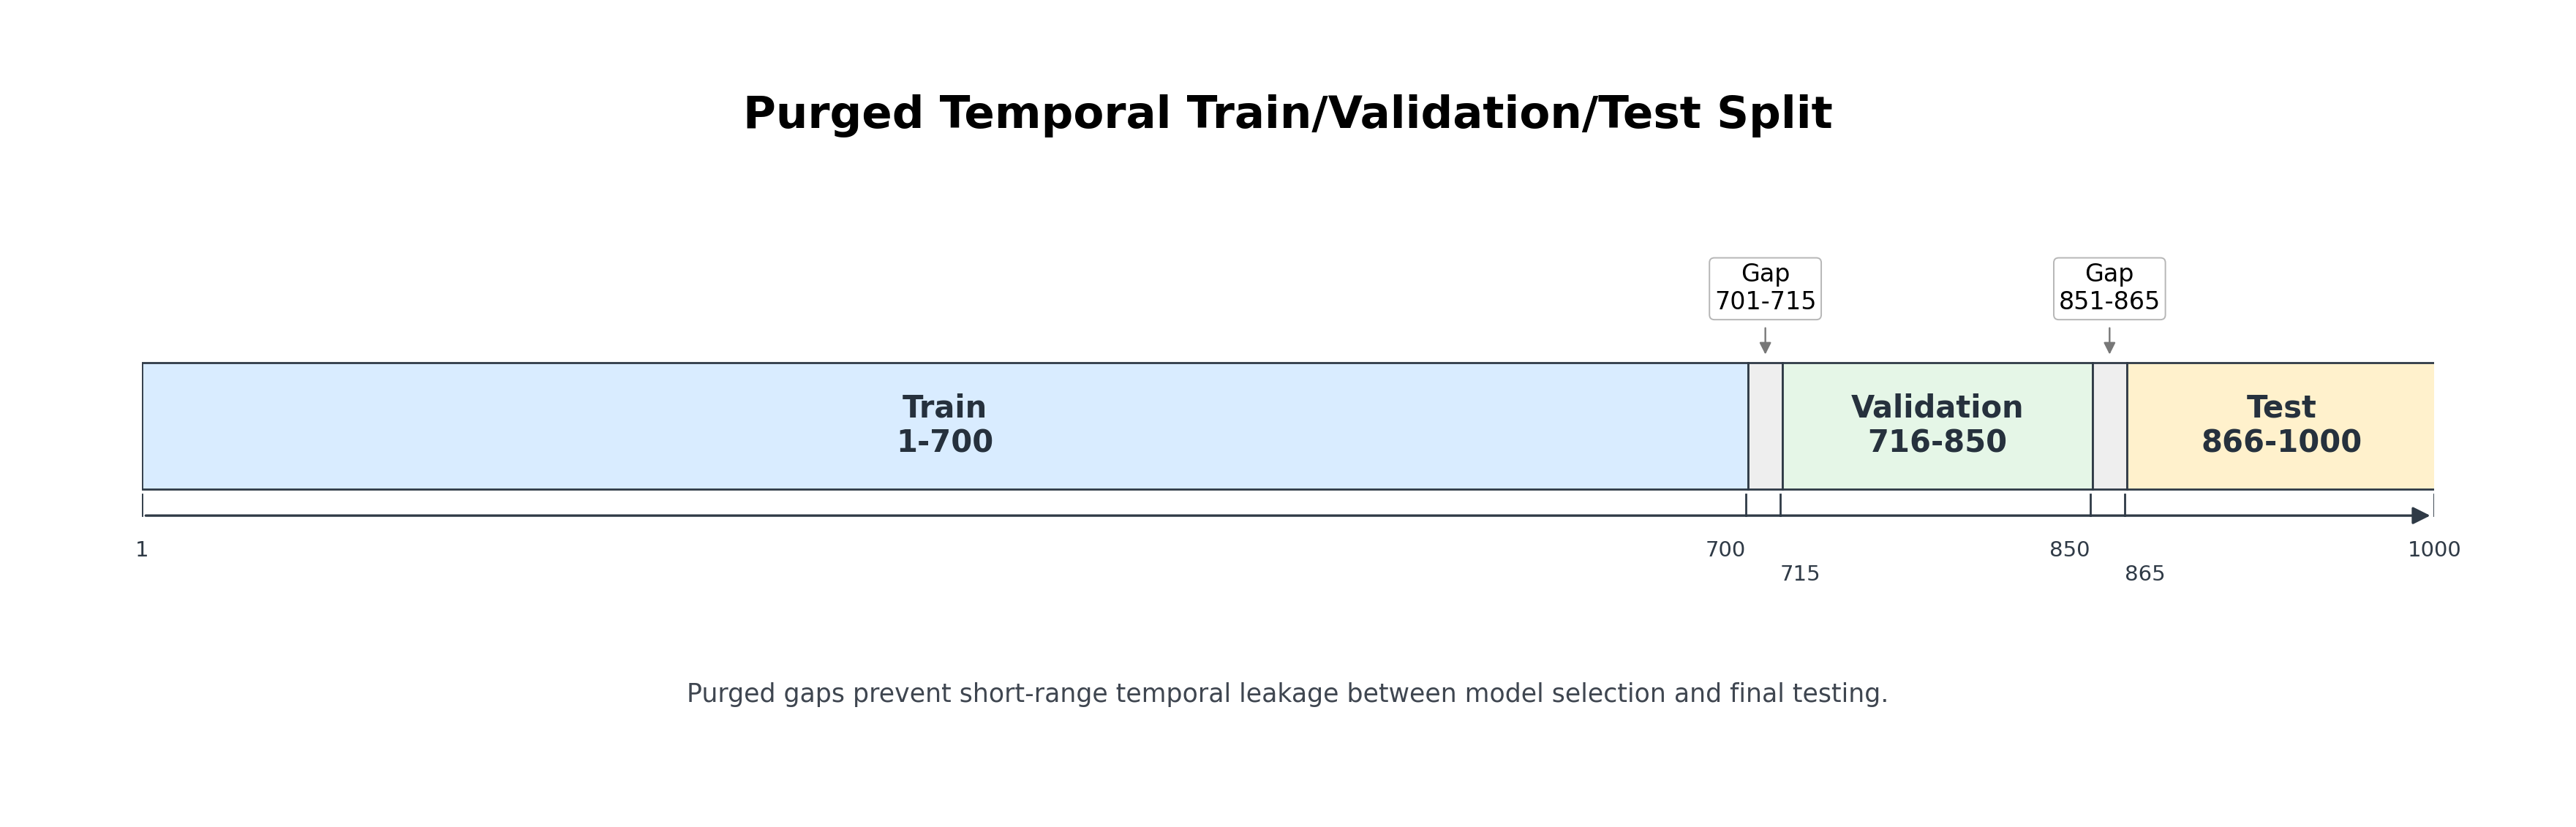
\includegraphics[width=\columnwidth]{figures/diagrams/151_fig_a2_temporal_split_protocol.png}
\caption{Purged temporal split used for model selection and final testing. Gap windows reduce near-boundary leakage between train, validation, and final test intervals.}
\label{fig:split_protocol_main}
\end{figure}

The temporal split is stricter than a random train/test split. It asks the policy to generalize forward in time, which is closer to deployment practice for workload traces. It also keeps the test split out of checkpoint selection. Validation is used for early stopping and model choice; the final test interval is used only for reporting.

For reproducibility, the dataset generator, six CSV files, temporal split definition, label-generation logic, analysis workflow, figure exporter, and manuscript figures are maintained as a single project package. The manuscript export bundle now includes a checksum manifest so future users can verify that their local CSV files match the benchmark used for the reported tables.

\subsection{Why the Dataset Changes the Evaluation}

In a dataset with mostly independent task rows, a model can perform well by learning a simple association between task size and destination. In \dataset{}, the same task can become edge-favorable or cloud-favorable depending on queue carryover, congestion state, outage state, local degradation, and cloud maintenance. This makes the offloading label less static. It also creates more ambiguous samples, which is why the latency-reference Oracle remains noticeably below the learned policy.

The dataset also makes rejection more meaningful. Corrupt tasks, deadline-admission flagged tasks, low-battery cases, and outage windows create situations where the selected action can be infeasible even when the other destination is not perfect. That failure mode is closer to a deployment scheduler: not every bad outcome is a high latency value; some tasks are rejected because the resource or state condition cannot support execution. The feature pipeline keeps these cases visible in the label and metric logic without letting sentinel latency values dominate model input.

\dataset{} functions as a controlled stress benchmark for algorithm comparison. It combines repeatable conditions with burst, fault, queue, and maintenance structure, making it suitable for evaluating offloading and resource-allocation decisions before future measured-trace or online-deployment studies.
